\documentclass[../../General.tex]{subfiles}
\begin{document}


\section{Identificación de usuarios}

El diseño y la implementación del robot autónomo para la medición de variables climáticas involucra a diversos actores dentro del ecosistema de una planta solar fotovoltaica a gran escala. Identificar a estos usuarios y comprender sus necesidades específicas es fundamental para establecer los requerimientos de diseño del sistema mecatrónico. Los agentes involucrados se clasifican en usuarios directos e indirectos.

Para estructurar visualmente el nivel de interacción de cada actor con el equipo y sus datos, se emplea un Stakeholder Map basado en un modelo concéntrico (ver Figura \ref{fig:StakeholderMap}). Esta herramienta clasifica a los agentes en tres niveles de proximidad: el núcleo operativo, el entorno comercial y de gestión y la periferia normativa e institucional.

    	\begin{figure}[H]
	\captionsetup{justification=raggedright, singlelinecheck=false, labelsep=none}
	
	\caption[Stakeholder Map con usuario principal, usuarios directos e indirectos]{} 
	
	\textit{Stakeholder Map con usuario principal, usuarios directos e indirectos} \par\medskip
	
	\centering
	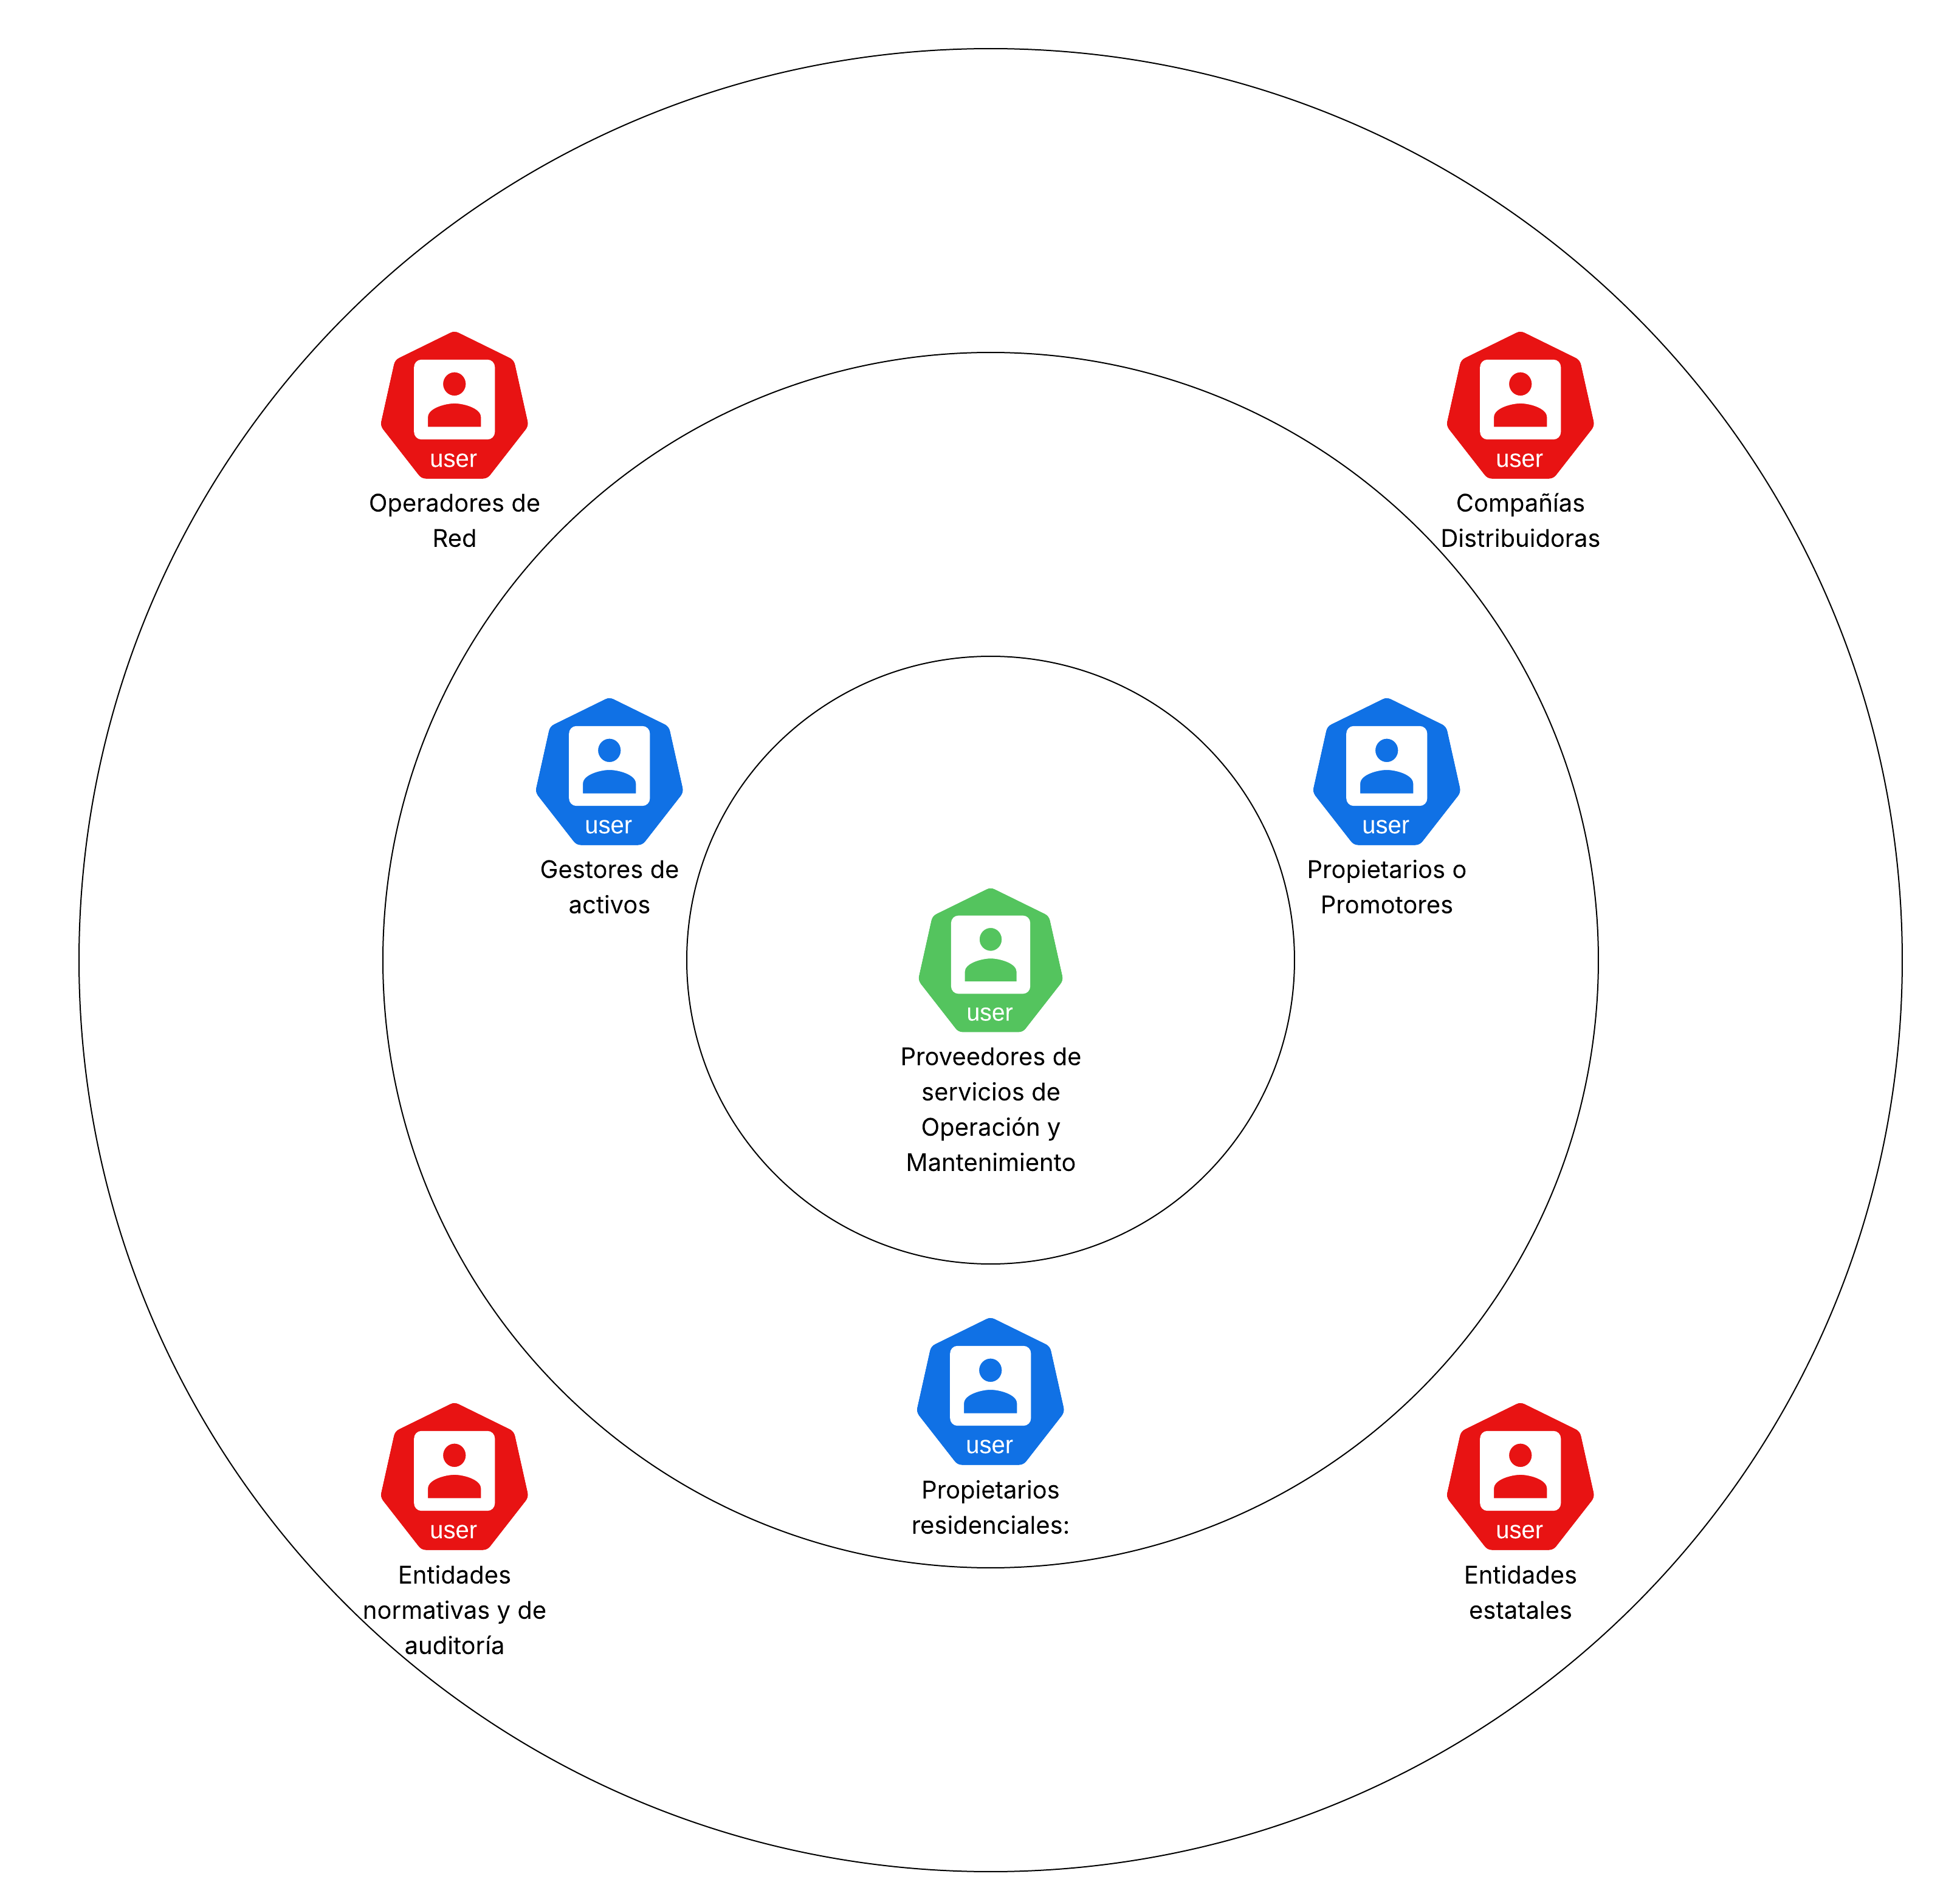
\includegraphics[width=\textwidth]{Recursos/Imagenes/Otros/StakeholderMap.png} \par\medskip
	
	\raggedright
	\footnotesize \textit{Nota.} Elaboración propia.
	\label{fig:StakeholderMap}
\end{figure}

\subsection{Usuario principal}

El usuario principal es aquel cuyas necesidades sirven como base principal de los requerimientos del proyecto.
\begin{itemize}
	
	
 \item \textbf{Proveedores de servicios de Operación y Mantenimiento (O\&M):} Personal técnico y de ingeniería encargado del funcionamiento diario de la planta. Su necesidad principal es transicionar de un enfoque de mantenimiento correctivo a uno predictivo y preventivo. Además, necesitan capturar datos climáticos precisos para cuantificar objetivamente las pérdidas por ensuciamiento y optimizar así sus ciclos de limpieza \citep{TesisJGB}.
\end{itemize}

\subsection{Usuarios directos}
Estos usuarios interactúan directamente con los datos generados por el sistema o dependen de ellos para la gestión técnica y comercial de la planta:

\begin{itemize}

    
    \item \textbf{Gestores de activos}: Profesionales o entidades responsables de la gestión comercial y financiera de la inversión en energía renovable, así como de la supervisión y control de las actividades técnicas delegadas a los contratistas de O\&M. Para llevar a cabo su labor de auditoría, requieren que la recolección de datos capture la variabilidad climática adecuada en el terreno. Esto les permite evaluar la salud de los activos, calcular con exactitud los indicadores clave de rendimiento, y comparar de forma objetiva si el rendimiento energético medido en el parque cumple con las expectativas de diseño \citep{ProyectoEjecutivo2024}.
    
    \item \textbf{Propietarios o Promotores}: Entidades inversoras o corporaciones dueñas de la instalación fotovoltaica que financian y promueven el proyecto desde su concepción. Su necesidad principal es salvaguardar la viabilidad del proyecto a largo plazo, reducir costos y prolongar la vida útil de los equipos para maximizar la rentabilidad de la infraestructura. Para ellos, disponer de mediciones climáticas dinámicas y representativas se traduce en una reducción de la incertidumbre operativa y financiera, garantizando que el retorno de inversión esté respaldado por datos confiables sobre el recurso solar\citep{ProyectoEjecutivo2024}.
    
    \item \textbf{Propietarios residenciales (Personas naturales)} : Representan a los individuos que poseen plantas fotovoltaicas personales, ya sean sistemas de generación distribuida orientados al autoconsumo o sistemas \textit{off-grid}. Aunque estas instalaciones operan a una escala mucho menor enfocada en la microgeneración, estos usuarios comparten la necesidad de contar con sistemas de medición accesibles que les permitan contrastar las variables climáticas locales con la producción de sus módulos. 
\end{itemize}

\subsection{Agentes indirectos}
Estos actores imponen las condiciones y los estándares de calidad bajo los cuales los datos del robot deben ser recolectados y transmitidos:

\begin{itemize}

    \item \textbf{Operadores de Red:} Entidades encargadas de la gestión de la red eléctrica nacional o regional. Necesitan que la planta fotovoltaica garantice una inyección de potencia predecible. La recolección dinámica de datos climáticos ayuda a prever fluctuaciones en la generación, permitiendo que los sistemas de control regulen adecuadamente la potencia activa y reactiva en el punto de interconexión (Kenemora Solar, 2024).
    
    \item \textbf{Compañías Distribuidoras:} Entidades encargadas de la facturación, los contratos y atención al cliente tanto a pequeña como mediana escala. Su principal interés es conocer al detalle el costo de la energía eléctrica para poder generar contratos mutuamente beneficiosos para ambas partes. En este sentido, las fluctuaciones en la generación ocasionan fuertes cambios en el costo de la energía, a veces sin posibilidad de modificar el costo que paga el cliente.
    
    \item \textbf{Entidades estatales:} El Comité de Operación Económica del Sistema (COES) tiene la misión de planificar la generación de cada una de las plantas, y asegurarse de que no haya un desbalance entre la energía generada y consumida por la ciudad. Para cumplir con este objetivo, requiere predicciones precisas de parte de las plantas renovables en la producción, para poder ordenar con precisión a las plantas no renovables los rangos de potencia a producir.
    
    \item \textbf{Entidades normativas y de auditoría técnica:} Organismos internacionales e independientes que establecen los estándares de calidad. Imponen la necesidad de que los datos recolectados posean trazabilidad, exactitud comprobable e instrumentación validada, de modo que los diagnósticos y las pruebas de evaluación de capacidad de la planta tengan total validez legal frente a terceros. Esto obliga a que el sistema se adhiera rigurosamente a estándares internacionales como la norma IEC 61724-1 para la monitorización general, y la IEC TS 61724-2 para los métodos de evaluación de capacidad.

\end{itemize}


\end{document}